\begin{appendices}
%\addappheadtotoc

\chapter{Intrabundle Usage}

\section{Setup environment}

In this work we provide a customized Forge distribution. This distribution downloads Intrabundle from its source code repository and automatically installs it in Forge environment when Forge is started.

The only prerequisite is to have JAVA\_HOME environment system variable pointing to a Java 6 or higher installation. Below are the steps to install Intrabundle and Forge:


\begin{enumerate}
\item Download Intrabundle Forge distribution from sourceforge: \\ \href{http://sourceforge.net/projects/intrabundle/files/latest/download}{http://sourceforge.net/projects/intrabundle/files/latest/download};
\item unzip it to a folder, i will call it HOME in this tutorial;
\item execute \emph{HOME/bin/forge} file if you are on Linux or MacOS, \\on Windows execute  \emph{HOME\textbackslash{}bin\textbackslash{}forge.bat} file;
\item you should see image \ref{forge start} and image \ref{intrabundle installation} as below:
\begin{figure}[h]
\caption{Forge start}
\label{forge start}
\centering
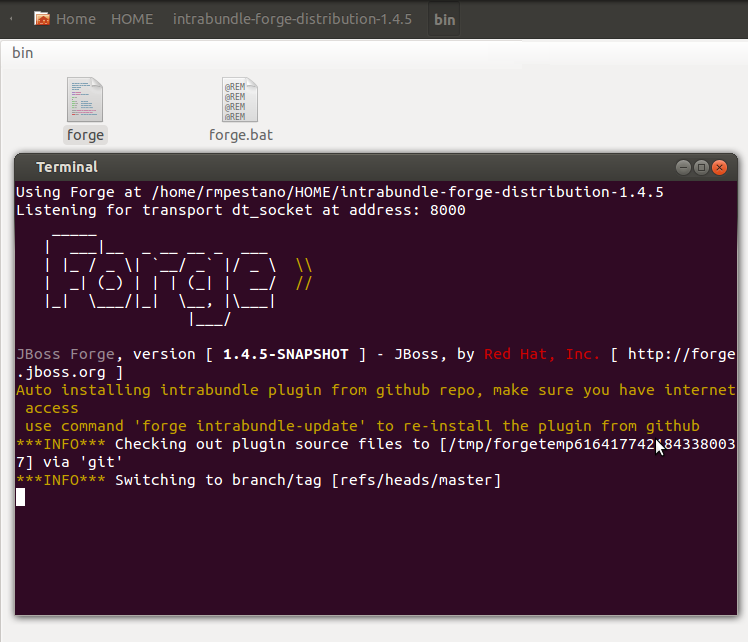
\includegraphics[scale=0.5]{tutorial01}
\end{figure}
\FloatBarrier

Intrabundle should be installed from its online source code repository, make sure you have internet access during this process:

\begin{figure}[h]
\caption{Intrabundle installation}
\label{intrabundle installation}
\centering
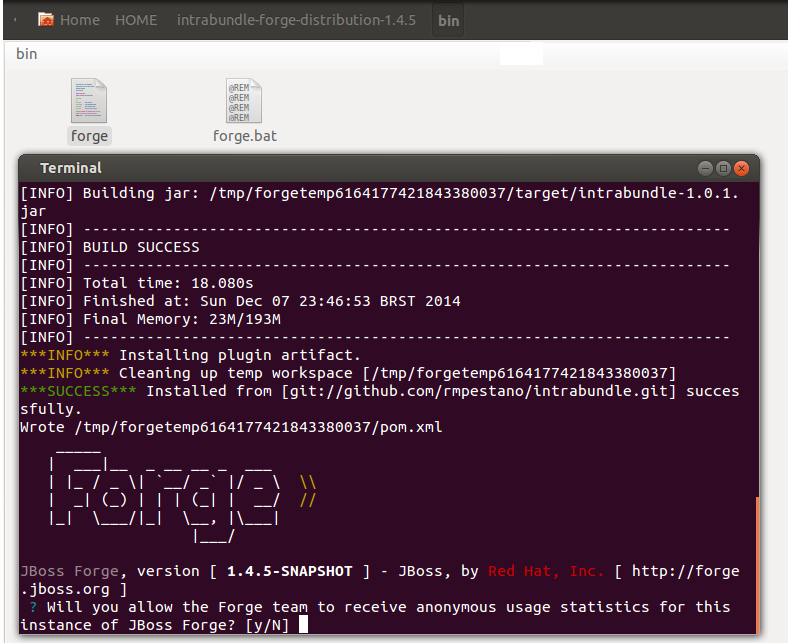
\includegraphics[scale=0.5]{tutorial02}
\end{figure}
\FloatBarrier
\end{enumerate}

There is also an online video you can watch to get you started with Intrabundle, see \citep{intrabundle github 2014}.

From now on you are ready to fire Forge and Intrabundle commands. 

\section{Begin Introspection}
With Forge up and running now you can start OSGi project introspection with Intrabundle. An example OSGi project can be found at \\
 \href{http://www.dcc.ufmg.br/\textasciitilde{}mtov/osgi\_example.zip}{http://www.dcc.ufmg.br/\textasciitilde{}mtov/osgi\_example.zip}, it is from the article \citep{Tavares 2008}.
Unzip the downloaded project to HOME and go back to Forge console.

Navigate to folder OSGI using \emph{cd} command: \emph{cd /HOME/OSGI}(you can use \emph{tab} for auto completion), like in Image \ref{navigate project}:

\begin{figure}[h]
\caption{Navigating to project}
\label{navigate project}
\centering
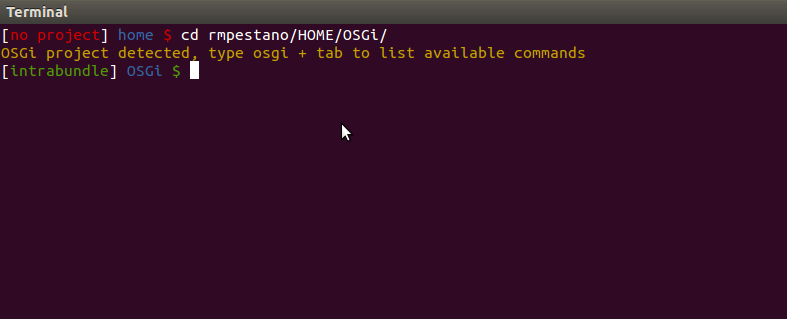
\includegraphics[scale=0.5]{tutorial03}
\end{figure}
\FloatBarrier
 
You can see that intrabundle recognized the OSGi project, so you can fire commands at OSGi project level like generate report or list bundles as well inspect its bundles, as in Image \ref{fire commands}:

\begin{figure}[h]
\caption{Fire commands}
\label{fire commands}
\centering
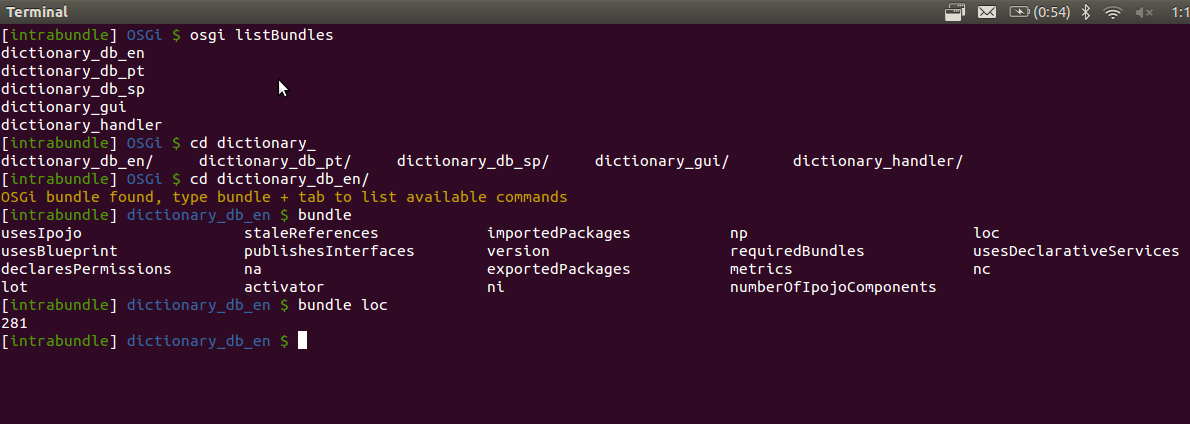
\includegraphics[scale=0.5]{tutorial04}
\end{figure}
\FloatBarrier

Another useful command Intrabundle provides is \emph{osgi-scan}, it search for OSGi bundles in file system and generate reports on top of them. To use it go back to HOME folder and fire \textbf{osgi-scan 2} command\footnote{number argument is the depth of folders to scan}, it must find bundles within downloaded project as is Image \ref{osgi-scan}:

\begin{figure}[h]
\caption{osgi-scan}
\label{osgi-scan}
\centering
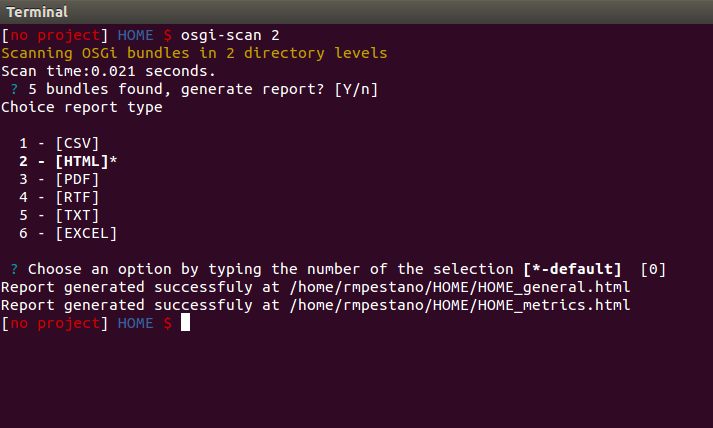
\includegraphics[scale=0.5]{tutorial05}
\end{figure}
\FloatBarrier

\chapter{Intrabundle Interfaces}
\label{ch:code-interfaces}

\section{OSGiProject}
\begin{lstlisting}[language=java,label=Intrabundle OSGiProject,caption=Intrabundle OSGiProject interface]
public interface OSGiProject extends Serializable{

    List<OSGiModule> getModules();

    Long getLinesOfCode();

    Long getLinesOfTestCode();

    Map<OSGiModule, List<OSGiModule>> getModulesDependencies();

    String getRevision();

    String getVersion();

    /**
     *
     * @return max quality point a project can have
     */
    int getMaxPoints();

}
\end{lstlisting}
\FloatBarrier

\section{OSGiModule}
\begin{lstlisting}[language=java,label=Intrabundle OSGiModule,caption=Intrabundle OSGiModule interface]
public interface OSGiModule extends Serializable, Comparable<OSGiModule>{

    /**
     *
     * @return total .java files(under src or src/main/java) lines of code
     */
    Long getLinesOfCode();


    /**
     * @return <code>true</code> if bundle uses declarative services specification
     * <code>false</code> if it doesnt
     */
    Boolean getUsesDeclarativeServices();

    /**
     * @return <code>true</code> if bundle uses Blueprint specification
     * <code>false</code> if it doesnt
     */
    Boolean getUsesBlueprint();

    /**
     *
     * @return object representing bundle MANIFEST.MF  or .bnd or pom.xml with maven-bundle-plugin
     */
    ManifestMetadata getManifestMetadata();

    /**
     *
     * @return bundle activator java file
     */
    FileResource<?> getActivator();

    /**
     *
     * @return bundle imported packages
     */
    List<String> getImportedPackages();

    /**
     *
     * @return bundle exported packages
     */
    List<String> getExportedPackages();

    /**
     *
     * @return bundle required bundles
     */
    List<String> getRequiredBundles();

    /**
     * @return <code>true</code> if bundle exported packages contains only interfaces
     * <code>false</code> if it has one or more classes
     */
    Boolean getPublishesInterfaces();

    /**
     *
     * @return <code>true</code> if bundle declares permissions
     * <code>false</code> otherwise
     */
    Boolean getDeclaresPermissions();

    /**
     *
     * @return .java files possibly containing OSGi service stale references
     */
    List<Resource<?>> getStaleReferences();
}
\end{lstlisting}
\FloatBarrier

\section{OSGiProject}
\begin{lstlisting}[language=java, caption=Intrabundle MetricsCalculator interface]
public interface MetricsCalculation {

    /**
     * this metric is based on bundle lines of code
     * its based on the fact that the less lines of code
     * the more cohesive the bundle is
     *
     * @param bundle
     * @return
     */
    Metric getLocMetric(OSGiModule bundle);


    /**
     * this metric is based on bundle dependencies
     * its based on the fact that the less bundle it
     * depends the less coupled it is
     *
     * @param bundle
     * @return
     */
    Metric getBundleDependencyMetric(OSGiModule bundle);


    Metric getPublishesInterfaceMetric(OSGiModule bundle);

    /**
     * verifies if bundle uses a framework to manage services lifecycle, frameworks being tracker are:
     * declarativeServices, bluePrint and ipojo
     *
     * @param bundle
     * @return Metric#STATE_OF_ART if use a framework,  Metric#REGULAR if no framework is used
     */
    Metric usesFrameworkToManageServicesMetric(OSGiModule bundle);

    Metric hasStaleReferencesMetric(OSGiModule bundle);

    Metric getDeclaresPermissionMetric(OSGiModule bundle);

    OSGiProject getCurrentOSGiProject();

    MetricPoints calculateBundleQuality(OSGiModule bundle);


    /**
     * get most frequent project metric score on current OSGiProject
     * @return
     */
    MetricScore calculateProjectModeQuality();

    /**
     * get absolute, based on percentage, project metric score on current OSGiProject
     * @return
     */
    MetricScore calculateProjectAbsoluteQuality();

    List<OSGiModule> getModulesByQuality(MetricScore quality);

    int getProjectQualityPonts();

    double getProjectQualityPointsPercentage();
}
\end{lstlisting}
\FloatBarrier


\end{appendices}
